\section{Results}
\label{sec:results}
\paragraph{Performance metrics}
\Cref{tab:scores-dialog} and \Cref{tab:scores-narration} show
the performance of several model configurations on the retrieval and
triplet tasks on the dialog and narration datasets respectively.

In the case of the narration data this scores is not confounded by
speaker-based clues, which is an indication that the model possibly
learned to detect some aspects of utterance meaning. We investigate
this hypothesis further using multiple representational similarity
analysis.
 

 \begin{table}
   \centering
   \begin{tabular}{rlrr}
\toprule
 ID & Pretraining &  Recall@10 &  Triplet Acc \\
\midrule
 43 &          AV &      0.193 &        0.814 \\
 44 &           V &      0.084 &        0.728 \\
 45 &        None &      0.034 &        0.597 \\
\bottomrule
\end{tabular}

   \caption{Retrieval and triplet scores on dialog validation data.}
   \label{tab:scores-dialog}
 \end{table}

\begin{table}
   \centering
   \begin{tabular}{rlrr}
\toprule
 ID & Pretraining &  Recall@10 &  Triplet Acc \\
\midrule
 43 &          AV &      0.239 &        0.866 \\
 44 &           V &      0.166 &        0.822 \\
 45 &        None &      0.087 &        0.741 \\
\bottomrule
\end{tabular}

   \caption{Retrieval and triplet scores on narration validation data.}
   \label{tab:scores-narration}
 \end{table}
 
\paragraph{Targeted Triplets}
\todo{add average targeted triplets result to general performance metrics table?}

We report results for the best performing model according to the
performance metrics (ID 48, audio and video pretraining). The average
targeted triplets accuracy is 0.679
. \Cref{fig:accuracy_targeted_triplets_nouns},
\Cref{fig:accuracy_targeted_triplets_verbs}, and
\Cref{fig:accuracy_targeted_triplets_adjectives} show per-word
accuracy for nouns, verbs, and adjectives, respectively. The vertical
bars indicate the standard deviation as estimated using bootstrapping
tests.
\todo{GC: It seems like we use resampling differently for the triplets
  (keep datapoints same, resample pairings) and
  the targeted triplets (resample datapoints) evaluation. Feasible to unify this?}

\begin{figure}
  \centering
  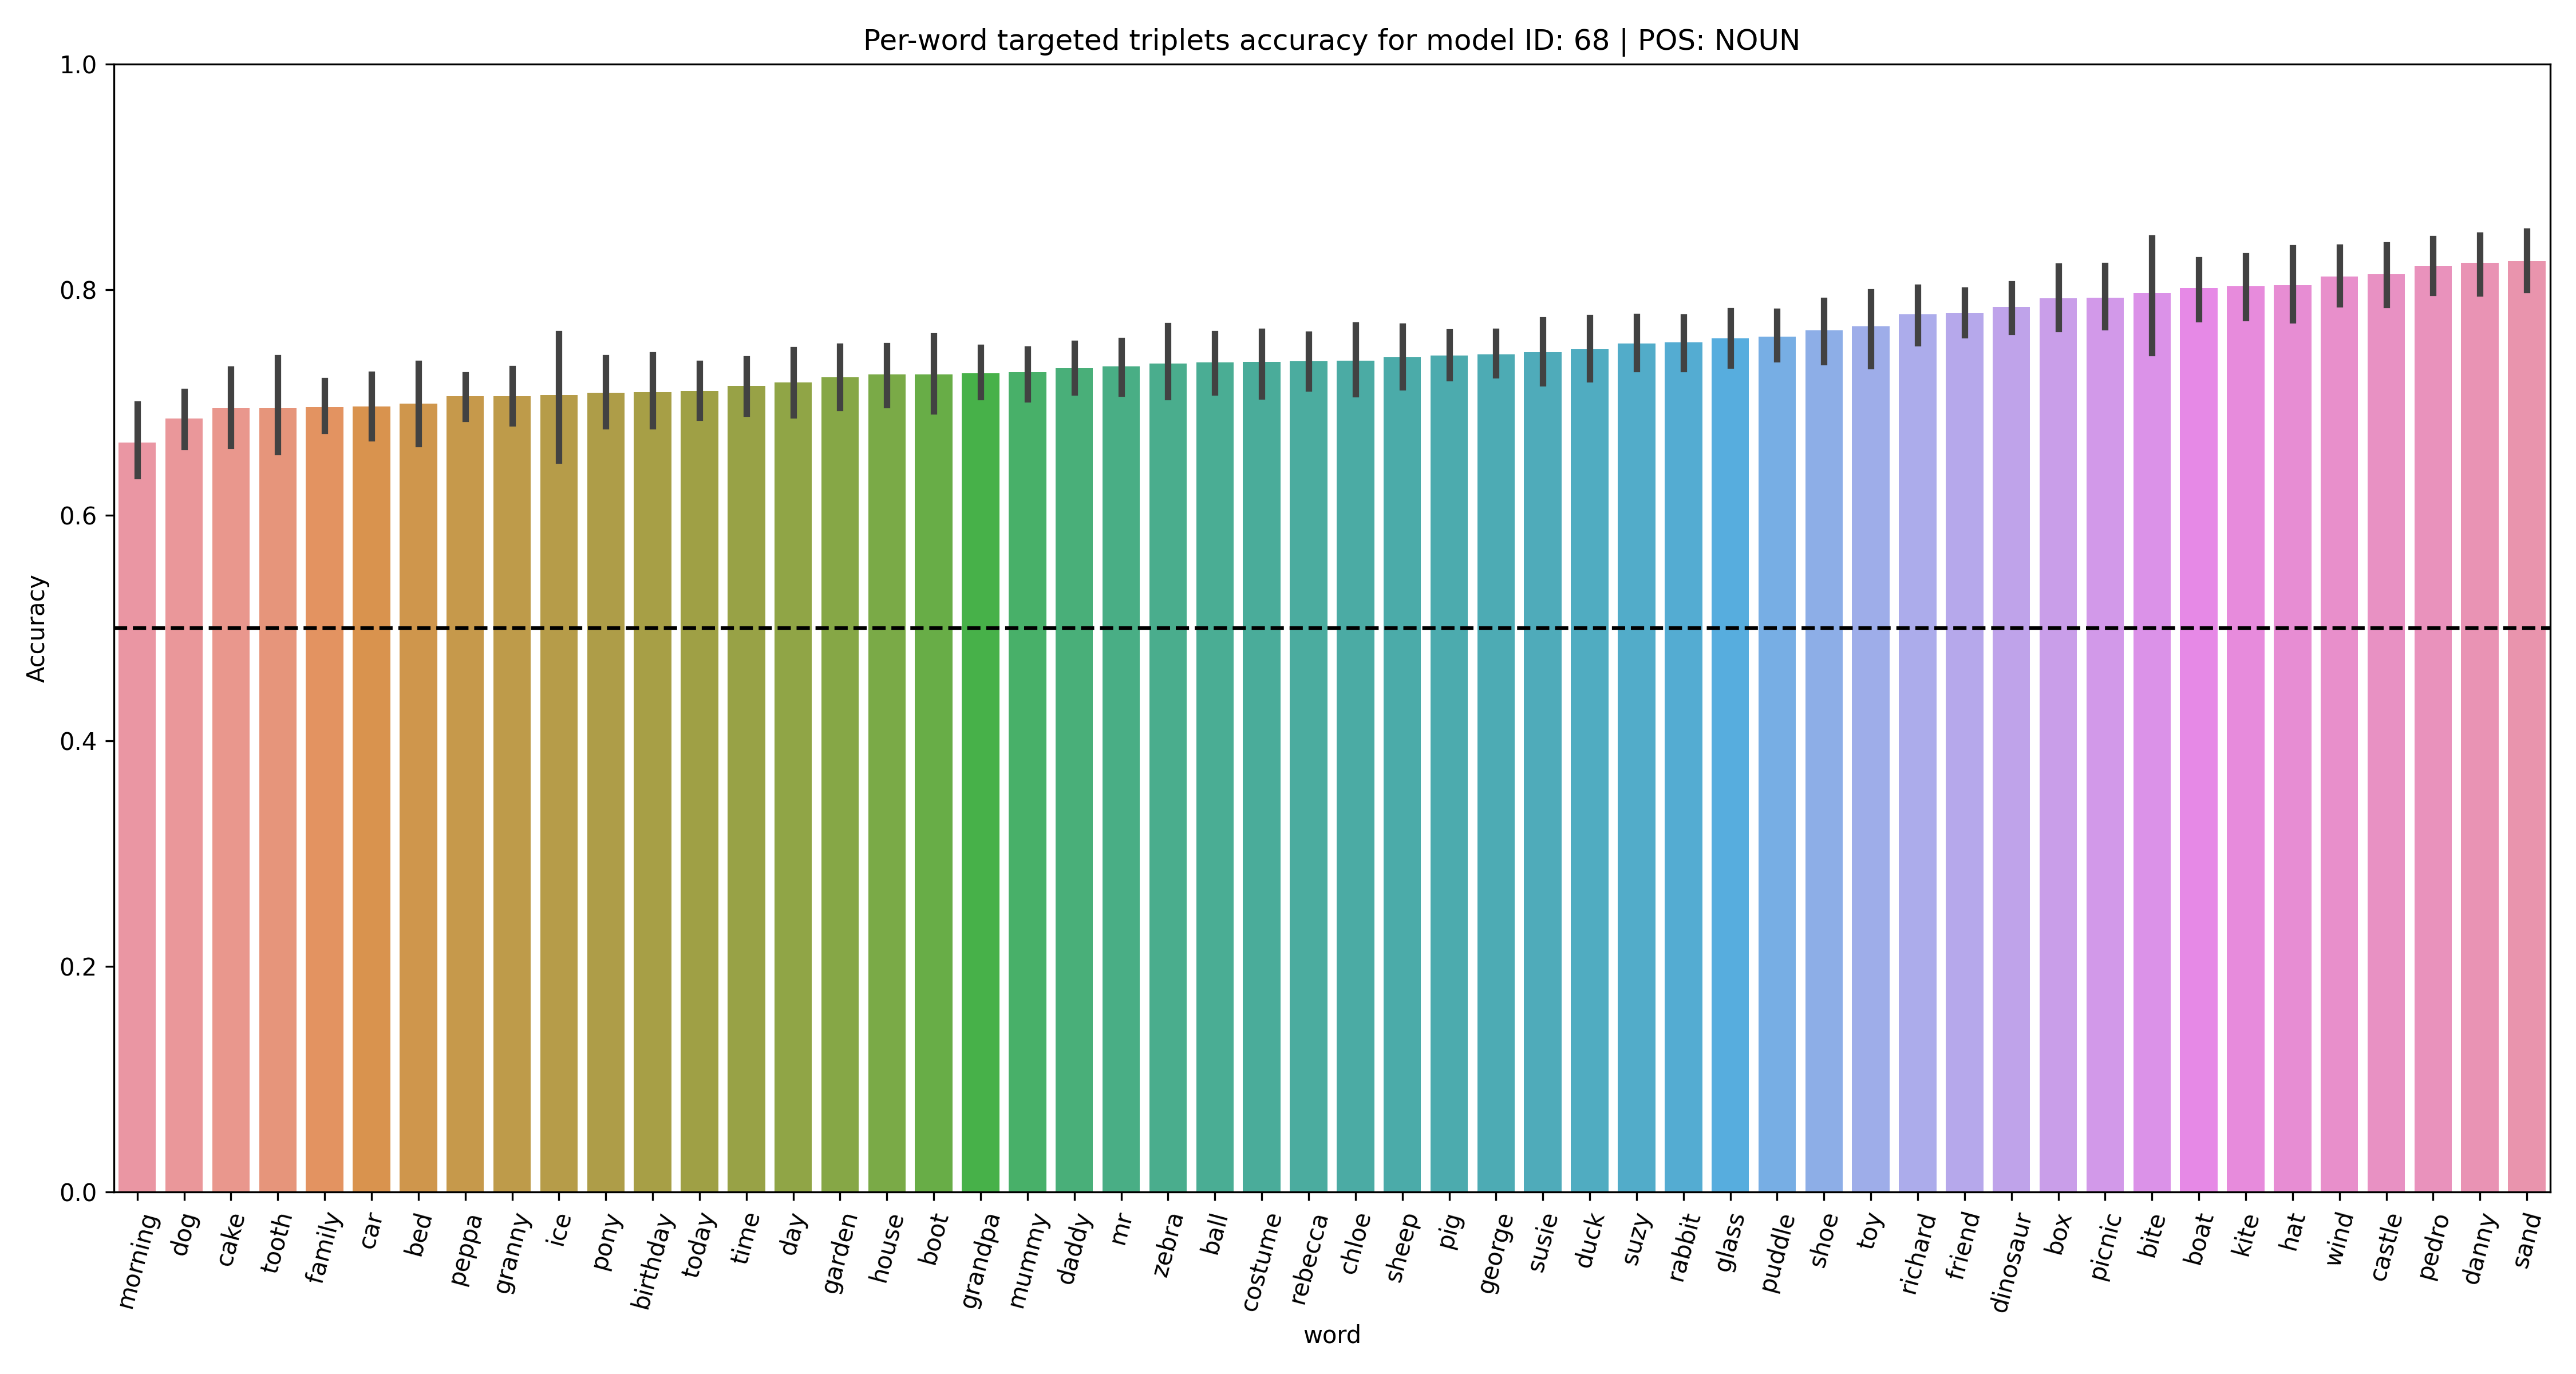
\includegraphics[width=\textwidth]{results/targeted_triplets/results_NOUN_word.png}
  \caption{Per-word targeted triplets accuracy for nouns.}
  \label{fig:accuracy_targeted_triplets_nouns}
\end{figure}

\begin{figure}
  \centering
  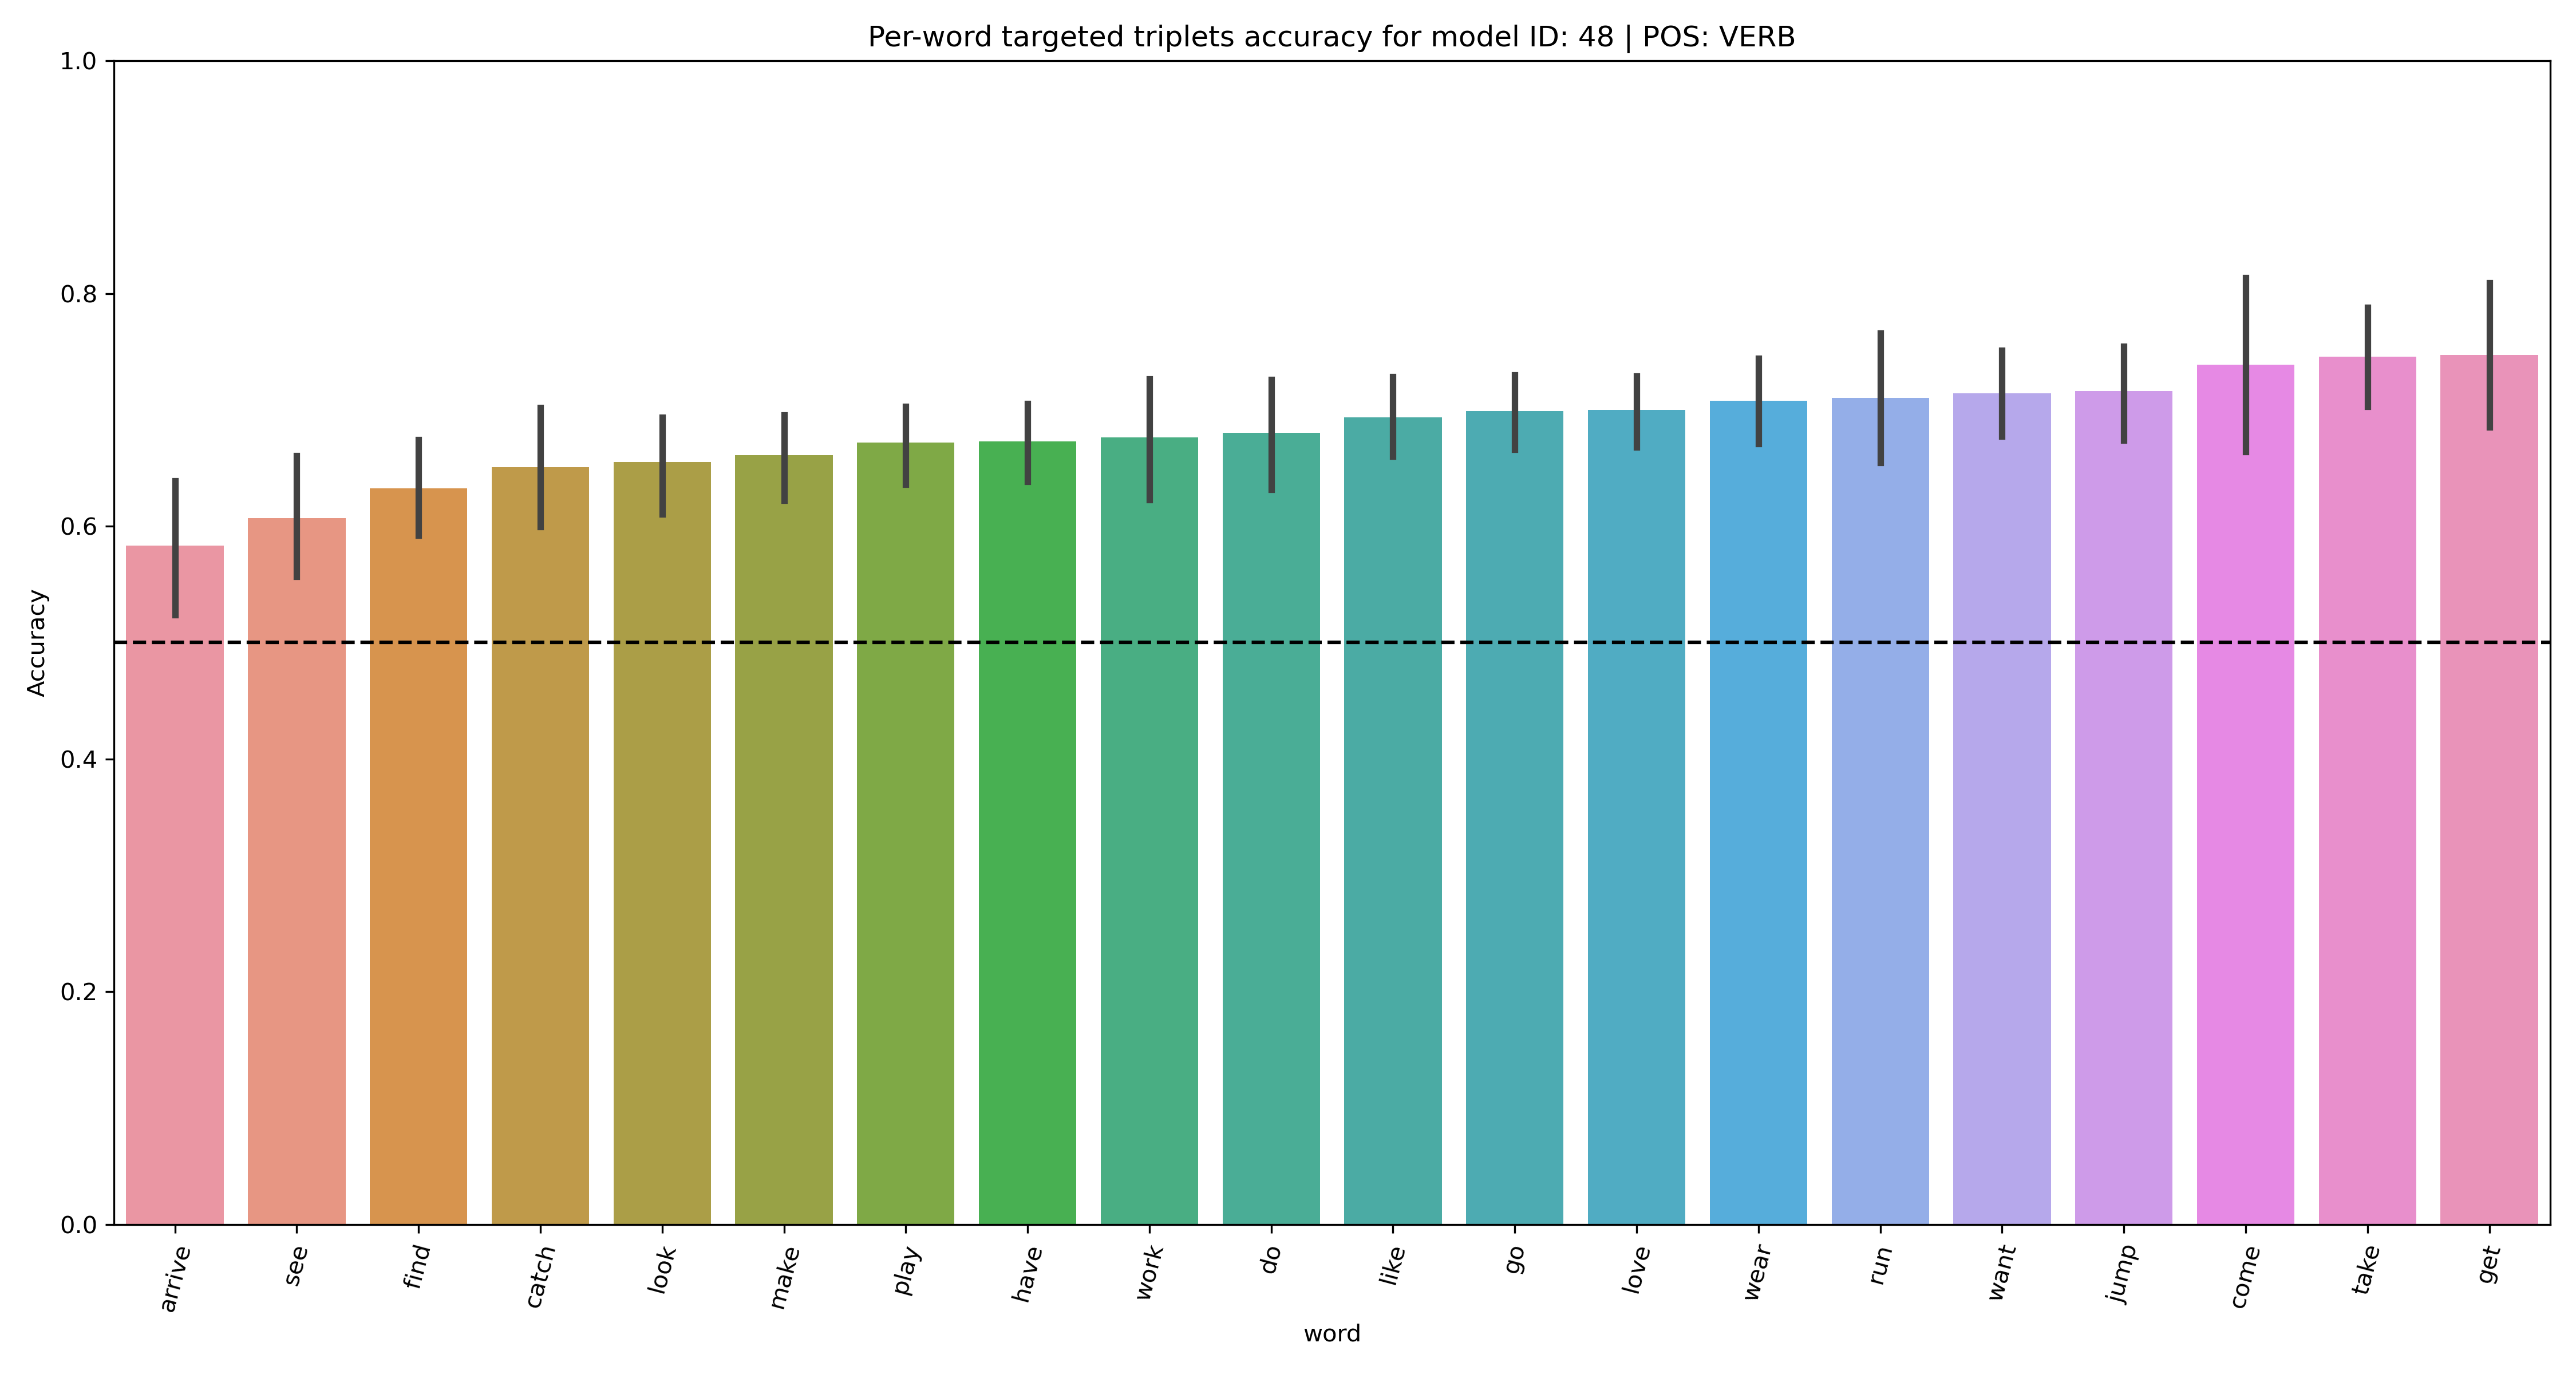
\includegraphics[width=\textwidth]{results/targeted_triplets/results_VERB_word.png}
  \caption{Per-word targeted triplets accuracy for verbs.}
  \label{fig:accuracy_targeted_triplets_verbs}
\end{figure}

\begin{figure}
  \centering
  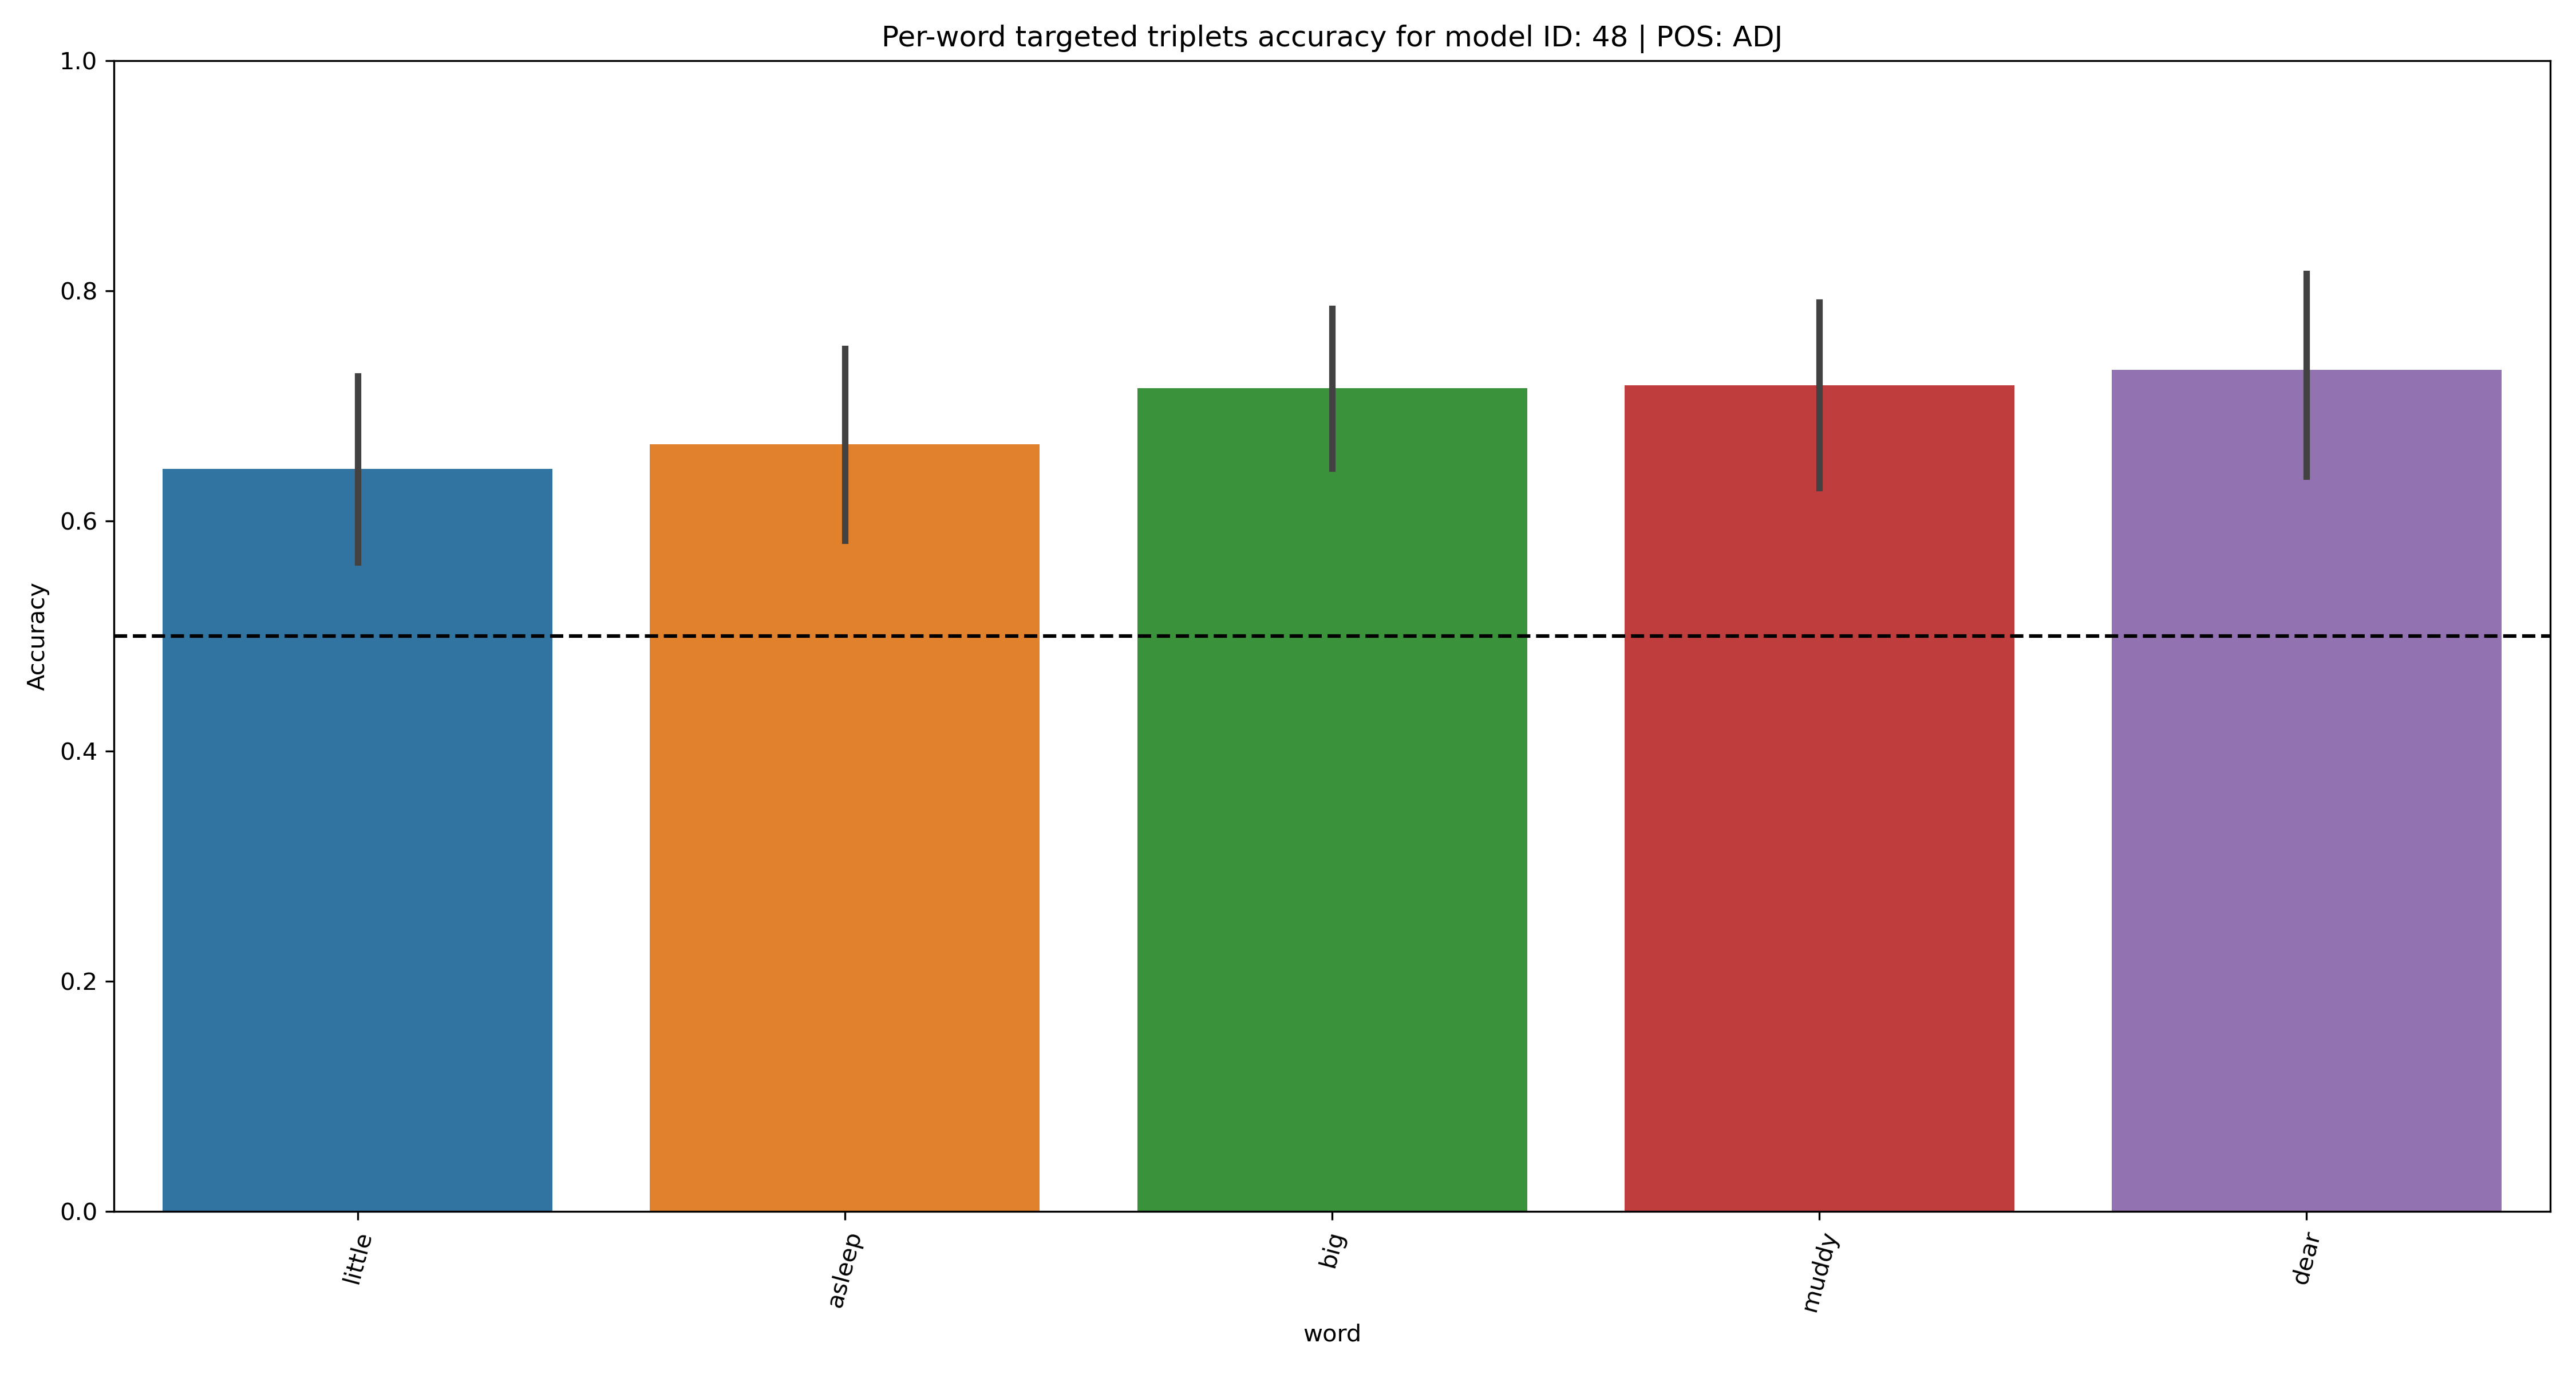
\includegraphics[width=\textwidth]{results/targeted_triplets/results_ADJ_word.png}
  \caption{Per-word targeted triplets accuracy for adjectives.}
  \label{fig:accuracy_targeted_triplets_adjectives}
\end{figure}

 
